\section{Introduction}
\label{sec:intro}

Reinforcement learning from verifiable rewards has become the standard way to
turn a base language model into a strong reasoner in one domain
\citep{shao2024deepseekmath,deepseek2025r1,yu2025dapo,he2025justrl,luo2025deepscaler}.
Because the reward is domain-specific, the result is a family of specialists
that share an initialization: from one base checkpoint, one model is trained
on competition mathematics, another on programming, a third on instruction
following \citep{olmo2025olmo3}. Each is far ahead on its own domain and far
behind on the others, so a user who wants mathematics and programming in the
same model has to build that model from the specialists.

\begin{figure}[t]
\centering
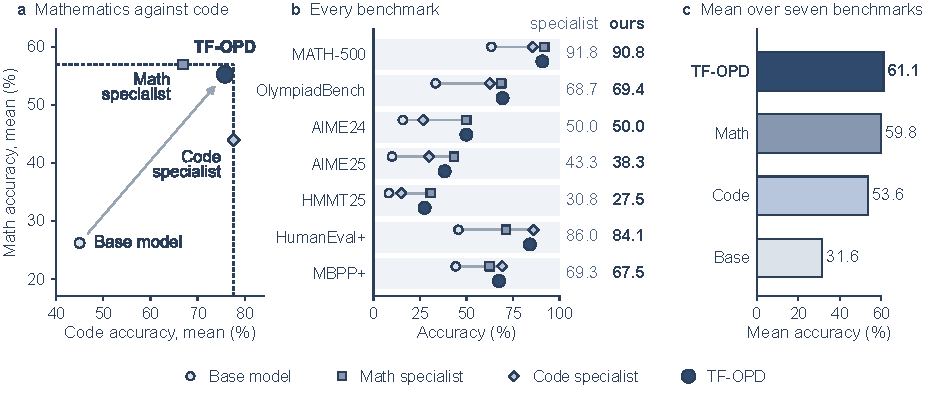
\includegraphics[width=\textwidth]{figs/results.pdf}
\caption{\textbf{A generalist with the highest mean accuracy, without
training (Olmo~3 7B).} (a)~Mean accuracy on the five mathematics benchmarks
against mean accuracy on the two code benchmarks; dashed lines mark what each
specialist reaches on its own domain, and \method, computed from the two with
forward passes only, lies next to the corner they define. (b)~Every
benchmark: the base model and the specialists on the upper line of each row,
\method below, and at the right the score of that domain's specialist and of
\method. (c)~Mean accuracy over the seven benchmarks: \method is more accurate
on average than either specialist it was built from.}
\label{fig:teaser}
\end{figure}

The available routes either train or ignore the rollouts
(Table~\ref{tab:routes}). One can repeat reinforcement learning on the union
of the domains \citep{liu2025prorl,liang2026boosting}, or distill: on-policy
distillation lets the student generate, has a teacher supervise those
generations, and updates the student on its own distribution
\citep{ross2011dagger,agarwal2024gkd,gu2024minillm}. It has become a
post-training route for consolidating specialists into one student
\citep{hou2026uniopd}, at the price of rollouts, teacher passes and gradient
steps for every teacher. The training-free alternative is to merge weights.
Arithmetic on parameters \citep{ilharco2023task} does not know which inputs
the parameters act on, and on reinforcement-learned specialists it can give
up part of what made them specialists: summing the mathematics and coding
updates of a 7B model leaves it below the mathematics specialist on AIME25
(Section~\ref{sec:exp-selection}). RegMean \citep{jin2023regmean} does use
inputs, in a closed-form least-squares solution, but takes them from each
task's training corpus, whereas a reasoning model spends almost all of its
computation on text it has generated itself.

\begin{table}[t]
\centering\small
\setlength{\tabcolsep}{8pt}
\begin{tabular}{@{}lccc@{}}
\toprule
Route & No training & On-policy inputs & Matches teachers \\
\midrule
Multi-domain RL             & $\times$     & $\checkmark$ & $\times$ \\
On-policy distillation      & $\times$     & $\checkmark$ & $\checkmark$ \\
Task arithmetic, TIES, DARE & $\checkmark$ & $\times$     & $\times$ \\
RegMean                     & $\checkmark$ & $\times$     & $\checkmark$ \\
\rowcolor{oursrow}[\tabcolsep][\tabcolsep]\method (ours) & $\checkmark$ & $\checkmark$ & $\checkmark$ \\
\bottomrule
\end{tabular}
\caption{\textbf{Routes from several specialists to one model.} \method needs
no training, gathers its statistics on text the models generate, and is fit
to match the specialists' outputs.}
\label{tab:routes}
\end{table}

We connect the two lines. For a single linear layer, asking the fused weight
to reproduce each teacher's output on that teacher's inputs is the
distillation objective restricted to the layer, and it is the least-squares
problem that RegMean solves: once the second moments of the inputs are known,
no optimization is left to run. \method gathers those moments where on-policy
distillation gathers its data, on rollouts. Each specialist answers a few
hundred training problems from its domain, the answers are filtered, the
specialist reads its kept answers once with teacher forcing while forward
hooks accumulate a Gram matrix per layer, and each layer is then solved
exactly. Nothing is back-propagated.

On Olmo~3 7B this yields a generalist without a single gradient step: one
model that keeps most of what each specialist gained on five mathematics and
two code benchmarks and that is, on average, more accurate than either
specialist alone (Figure~\ref{fig:teaser}).
Three findings explain when it
works. First, the filter carries the result. A minority of the mathematics
specialist's rollouts run to the length limit in a repetition loop: few among
the answers, several times more among the tokens. With them the closed form is
no better than task arithmetic on AIME25, and removing them alone closes the
gap to the specialist scored in the same format. Second, the token-level fit is
not what fails: the unfiltered model already follows the specialist almost
token for token, so hard problems are decided by which inputs the statistics
weigh. Third, rollouts written by the student, the on-policy data of trained
distillation, do not improve the closed form. Reinforcement learning also
moves weights so little that the 16-bit release format distorts a fused
update, which makes the formats of storage and evaluation part of the method.

\begin{figure}[t]
\centering
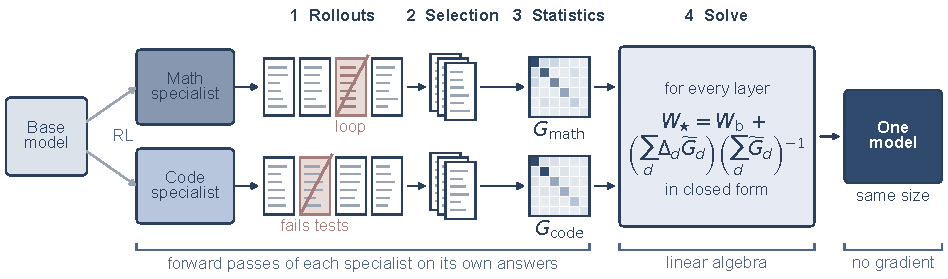
\includegraphics[width=\textwidth]{figs/overview.pdf}
\caption{\textbf{Overview of \method.} Two specialists trained from one base
model each answer training problems of their own domain~(1); answers that end
in a repetition loop or fail grading are dropped~(2); each specialist reads its
kept answers once while hooks record the second moments $G_d$ of every layer's
inputs~(3); and each layer of the fused model is obtained by one linear
solve~(4). Steps 1 to 3 are forward passes and step 4 is linear algebra, so no
gradient is computed at any point. Step 2 decides the hard problems
(Section~\ref{sec:selection}).}
\label{fig:overview}
\end{figure}

\needspace{6\baselineskip}
\paragraph{Contributions.}
\begin{itemize}
\item We show that the capabilities of separately tuned specialists can be
aggregated without training. On Olmo~3 7B, a closed-form fusion of a
mathematics and a coding specialist keeps most of each specialist's gain on
seven benchmarks and is, on average, more accurate than either specialist
alone, after a few GPU-hours of forward computation per specialist.
\item The method, \method, reads layer-wise distillation from several
teachers as the closed-form problem of RegMean and feeds it statistics from
the specialists' own rollouts, using forward passes only.
\item We show that the composition of those rollouts decides the outcome on
hard problems. Truncated answers ending in repetition loops are a small share
of answers and a large share of tokens, and removing them separates a fused
model that falls short of its mathematics specialist from one that matches it
in the same evaluation format.
\item We analyze what matters and what does not: a close token-level fit does
not protect hard problems; student rollouts, domain reweighting and mined
hard problems do not improve on selection; numerical precision does.
\end{itemize}
